\chapter{Electron-electron interaction in second quantization} \label{ch:4}

\section{The Coulomb repulsion Hamiltonian}
It was a great success that we solved the many-electron problem in
the self-consistent field approximation. The solutions exhibit important
physical quantities, such as the electron density distribution and the total energy of the system.
If someone asks us to summarize the spirit of the methods into one word,
then this word must be ``mean-field''. It was the mean-field potential
that simplified our problem dramatically.
However, by introducing a mean-field, we sacrificed detailed information
how exactly individual electrons interact among themselves.

Consider a carbon atom with electronic configuration: $1s^2$ $2s^2$ $2p^2$.
Both the $1s^2$ and $2s^2$ shells are fully occupied, but the $2p^2$ shell is
still open. According to the Pauli exclusion principle, one $p$ shell can contain
at most 6 electrons with orbital angular projection momentum $m=1,0,-1$ and spin angular
projection momentum $\sigma=\uparrow,\downarrow$.\footnote{A more general convention
is to write the orbital and spin projection quantum numbers as $m_l$ and $m_s$, respectively.
When a spin 1/2 particle (in our case electron) is considered,
we can also write them as $m$ and $\sigma$ to simplify our notations.}
Since the $2p^2$ shell is not fully occupied, these two electrons can take
different quantum numbers among those allowed $m$ and $\sigma$.
But how exactly are these two electrons arranged, our mean-field potential
does not tell a difference. In this $2p^2$ shell, energies of
different $m$ and $\sigma$ are all degenerate.

It is important to understand why the mean-field
potential distinguishes ``$n$ and $l$'' but not ``$m$ or $\sigma$'': Because we calculated
the mean-field potential according to electron radial wave functions $R_{nl}$, which
are distinguished by quantum numbers $n$ and $l$. But for the angular part,
we made an approximation that the electrons are spherical symmetrically
distributed, which implies all $Y_{lm}$ are treated equally as $Y_{00}$.
Moreover, we didn't make a distinction between spin up and spin down.
It doesn't really matter which $m$ or $\sigma$ state the electron is.
However, the real physics is, due to the interaction among electrons,
there will be an energy-splitting among different $m$ and $\sigma$ quantum states.
Since our mean-field potential cannot resolve this energy-splitting,
this might be a good time for us to revisit our ``trouble maker'':
the very complicated Coulomb repulsion potential
\begin{equation} \label{eq:U}
H_U = \sum_{i<j}^N \frac{1}{|\vec{r}_i - \vec{r}_j|}
\end{equation}
%
Previously we replaced this electron-electron repulsion by a mean-field potential.
Now, we would like to handle it directly, which is, of course, not easy.
This Coulomb repulsion Hamiltonian becomes more handleable if we reformulate it
into second quantization (see Appendix~\ref{app:B})
\begin{equation} \label{eq:U2nd}
H_U = \frac{1}{2} \sum_{\alpha,\beta,\gamma,\delta} U_{\alpha\beta\gamma\delta} c_\alpha^\dag c_\beta^\dag c_\gamma c_\delta
\end{equation}
where,
\begin{align}
\alpha & = \{n_1,\,l_1,\,m_1,\,\sigma_1\} \nonumber \\
\beta  & = \{n_2,\,l_2,\,m_2,\,\sigma_2\} \nonumber \\
\gamma & = \{n_3,\,l_3,\,m_3,\,\sigma_3\} \nonumber \\
\delta & = \{n_4,\,l_4,\,m_4,\,\sigma_4\} \nonumber
\end{align}
%
These four indices $(\alpha,\beta,\gamma,\delta)$ represent four sets of electron
quantum numbers. Perhaps the immediate question is,
``Why four indices?'' It seems like we need only two indices since each electron-pair
interaction in Eqn.~(\ref{eq:U}) involves two electrons.
In Eqn.~(\ref{eq:U2nd}), we have two electron creators and two electron annihilators.
If we understand the mechanism of those creation and annihilation operators,
this picture will become much clearer. Let's say initially we have a two-electron state
$\Ket{\gamma,\delta}$. First, the operator $c_\delta$
annihilates the electron with quantum number $\delta$, which
produces $\Ket{\gamma}$. Then, $c_\gamma$ annihilates the second
electron and returns a vacuum state $\Ket{0}$. Next, the creation operator
$c_\beta^\dag$ creates an electron from the vacuum and we get $\Ket{\beta}$.
Finally, $c_\alpha^\dag$ creates another electron and we obtain our final state
$\Ket{\beta,\alpha}$.
\begin{equation*}
\Ket{\gamma,\delta}
\stackrel{c_\delta}{\longrightarrow}
\Ket{\gamma}
\stackrel{c_\gamma}{\longrightarrow}
\Ket{0}
\stackrel{c_\beta^\dag}{\longrightarrow}
\Ket{\beta}
\stackrel{c_\alpha^\dag}{\longrightarrow}
\Ket{\beta,\alpha}
\end{equation*}
%
This four-step process involves two electrons. One can think
$\Ket{\gamma,\delta}$ as the initial state and
$\Ket{\beta,\alpha}$ as the final state.
That is why four indices are involved.

The next question is, ``What's the range of the indices?'' The answer is that
the indices enumerate all possible quantum states of electrons, that is, infinitely many.
In fact, Eqn.~(\ref{eq:U2nd}) is absolutely equivalent to Eqn.~(\ref{eq:U}).
They are just two different formulations on the same physics problem.
But later we need to restrict the range of the indices,
say, into the same shell, making an approximation.
Otherwise the dimension of the problem will be too huge to be solvable.
The very important $U_{\alpha\beta\gamma\delta}$ is called the matrix element,
from which we see the connection between Eqns.~(\ref{eq:U}) and (\ref{eq:U2nd}).
\begin{equation} \label{eq:Umat}
U_{\alpha\beta\gamma\delta} =
\delta_{\sigma_1\sigma_4} \delta_{\sigma_2\sigma_3} \int d^3r_1 \int d^3r_2 \,
\conj{\varphi_{n_1l_1m_1}}(\vec{r}_1) \conj{\varphi_{n_2l_2m_2}}(\vec{r}_2)
\frac{1}{|\vec{r}_1 - \vec{r}_2|}
\varphi_{n_3l_3m_3}(\vec{r}_2) \varphi_{n_4l_4m_4}(\vec{r}_1)
\end{equation}
%
$U_{\alpha\beta\gamma\delta}$ is really just a ``number''. But the multi-dimensional
integration makes the computation not trivial at all. In fact, this entire chapter
is dedicated to discussing the computation of this Coulomb repulsion matrix element,
which plays a crucial role in our problem. The difficulty of evaluating this integral
comes from the fact that $\vec{r}_1$ and $\vec{r}_2$ are coupled together.
I admit that the term $\frac{1}{|\vec{r}_1 - \vec{r}_2|}$ looks lovely.
But we cannot go further if this coupling term exists. Unfortunately,
we have to expand this lovely term into a monster. It is called the
multipole expansion \cite{YBE}
\begin{equation} \label{eq:multExp}
\frac{1}{|\vec{r}_1 - \vec{r}_2|} = \sum_{k=0}^\infty \frac{r_<^k}{r_>^{k+1}} \frac{4\pi}{2k+1}
                                    \sum_{\mu=-k}^k \conj{Y_{k\mu}}(\theta_1,\phi_1) Y_{k\mu}(\theta_2,\phi_2)
\end{equation}
If $r_1 \le r_2$,
\begin{equation} \label{eq:r1lr2}
  \begin{array}{c c}
  r_<=r_1, & r_>=r_2
  \end{array}
\end{equation}
If $r_1 > r_2$,
\begin{equation} \label{eq:r1gr2}
  \begin{array}{c c}
  r_<=r_2, & r_>=r_1
  \end{array}
\end{equation}
%
The magic of Eqn.~(\ref{eq:multExp}) is that it separates $\vec{r}_1$ and $\vec{r}_2$.
In other words, $(r_1,\theta_1,\phi_1)$ and $(r_2,\theta_2,\phi_2)$ can be integrated independently.
Now, we want to substitute (\ref{eq:multExp}) into (\ref{eq:Umat}).
Er... well, maybe we could do some abbreviation first to reduce our headache.
The multipole expansion consists of two major parts:

The radial part,
\begin{align} \label{eq:radPart}
R^{(k)}(n_1l_1,n_2l_2,n_3l_3,n_4l_4) & = \int_0^\infty dr_1\,r_1^2 \int_0^\infty dr_2\,r_2^2\, \conj{R_{n_1l_1}}(r_1) \conj{R_{n_2l_2}}(r_2)
                                     \frac{r_<^k}{r_>^{k+1}} R_{n_3l_3}(r_2) R_{n_4l_4}(r_1) \nonumber \\
& = \int_0^\infty dr_1 \int_0^\infty dr_2\, \conj{u_{n_1l_1}}(r_1) \conj{u_{n_2l_2}}(r_2)
    \frac{r_<^k}{r_>^{k+1}} u_{n_3l_3}(r_2) u_{n_4l_4}(r_1)
\end{align}
%
The angular part,
\begin{align} \label{eq:angPart}
A^{(k)}(l_1m_1,l_2m_2,l_3m_3,l_4m_4) = \sum_{\mu=-k}^k
& \int_0^{2\pi}d\phi_1 \int_0^{\pi}d\theta_1\,\sin{\theta_1}\,
  \conj{Y_{l_1m_1}}(\theta_1,\phi_1) \conj{Y_{k\mu}}(\theta_1,\phi_1) Y_{l_4m_4}(\theta_1,\phi_1) \nonumber \\
& \int_0^{2\pi}d\phi_2 \int_0^{\pi}d\theta_2\,\sin{\theta_2}\,
  \conj{Y_{l_2m_2}}(\theta_2,\phi_2) Y_{k\mu}(\theta_2,\phi_2) Y_{l_3m_3}(\theta_2,\phi_2)
\end{align}
%
Consequently, Eqn.~(\ref{eq:Umat}) can be written as
\begin{equation} \label{eq:UmatExp}
\boxed{
U_{\alpha\beta\gamma\delta} =
\delta_{\sigma_1\sigma_4} \delta_{\sigma_2\sigma_3}
\sum_{k=0}^\infty \frac{4\pi}{2k+1} R^{(k)}(n_1l_1,n_2l_2,n_3l_3,n_4l_4)
A^{(k)}(l_1m_1,l_2m_2,l_3m_3,l_4m_4)
}
\end{equation}
Hum... Much clearer. But the difficulty remains: how to evaluate the radial part
$R^{(k)}(n_1l_1,n_2l_2,n_3l_3,n_4l_4)$ and the angular part $A^{(k)}(l_1m_1,l_2m_2,l_3m_3,l_4m_4)$,
respectively?

\section{Slater-Condon parameters}
Our first task is to solve the radial part:
\begin{equation} \label{eq:Rk}
R^{(k)}(n_1l_1,n_2l_2,n_3l_3,n_4l_4) =
\int_0^\infty dr_1 \int_0^\infty dr_2\, \conj{u_{n_1l_1}}(r_1) \conj{u_{n_2l_2}}(r_2)
\frac{r_<^k}{r_>^{k+1}} u_{n_3l_3}(r_2) u_{n_4l_4}(r_1)
\end{equation}
%
But how is it possible to evaluate such an integral with those mysterious $r_<$
and $r_>$? Recall how they are defined in Eqns.~(\ref{eq:r1lr2}) and (\ref{eq:r1gr2}).
We note down,

If $r_1 \le r_2$,
\begin{equation}
\frac{r_<^k}{r_>^{k+1}} = \frac{r_1^k}{r_2^{k+1}}
\end{equation}
If $r_1 > r_2$,
\begin{equation}
\frac{r_<^k}{r_>^{k+1}} = \frac{r_2^k}{r_1^{k+1}}
\end{equation}
%
Hum... it appears not that scary now. And the integration below can be evaluated casewise:
\begin{align} \label{eq:r1r2Split}
  {} & \int_0^\infty dr_2\, \conj{u_{n_1l_1}}(r_1) \conj{u_{n_2l_2}}(r_2)
       \frac{r_<^k}{r_>^{k+1}} u_{n_3l_3}(r_2) u_{n_4l_4}(r_1) \nonumber \\
= {} & \int_0^{r_1} dr_2\, \conj{u_{n_1l_1}}(r_1) \conj{u_{n_2l_2}}(r_2)
       \frac{r_2^k}{r_1^{k+1}} u_{n_3l_3}(r_2) u_{n_4l_4}(r_1)
       + \int_{r_1}^\infty dr_2\, \conj{u_{n_1l_1}}(r_1) \conj{u_{n_2l_2}}(r_2)
       \frac{r_1^k}{r_2^{k+1}} u_{n_3l_3}(r_2) u_{n_4l_4}(r_1) \nonumber \\
= {} & \conj{u_{n_1l_1}}(r_1)u_{n_4l_4}(r_1)
       \left[ \frac{1}{r_1^{k+1}} \int_0^{r_1} dr_2\, r_2^k \conj{u_{n_2l_2}}(r_2)u_{n_3l_3}(r_2)
       + r_1^k \int_{r_1}^\infty dr_2\, \frac{1}{r_2^{k+1}} \conj{u_{n_2l_2}}(r_2)u_{n_3l_3}(r_2) \right]
\end{align}
%
Hence, Eqn.~(\ref{eq:Rk}) reads
\begin{equation} \label{eq:RkSplit}
\boxed{
\begin{aligned}
& R^{(k)}(n_1l_1,n_2l_2,n_3l_3,n_4l_4) = \\
& \int_0^\infty dr_1
\conj{u_{n_1l_1}}(r_1)u_{n_4l_4}(r_1)
\left[ \frac{1}{r_1^{k+1}} \int_0^{r_1} dr_2\, r_2^k \conj{u_{n_2l_2}}(r_2)u_{n_3l_3}(r_2)
+ r_1^k \int_{r_1}^\infty dr_2\, \frac{1}{r_2^{k+1}} \conj{u_{n_2l_2}}(r_2)u_{n_3l_3}(r_2) \right]
\end{aligned}
}
\end{equation}
%
Absolutely under our control, not? We are glad to see that $r_1$ and $r_2$ are separated.
This is the Slater-Condon parameter that we are going to evaluate.
One should be aware that for a given index $\{n,l\}$, the radial wave
function $u_{nl}$ is not uniquely determined. It depends on the choice
of the system. For instance, one can use the hydrogen-like radial wave functions,
whose solutions are known analytically. But as a better estimation,
we will use the radial wave functions from our self-consistent
calculations. In fact, this ab-initio Slater-Condon parameter
enters as a connection between our previous results
and the multiplet calculations that we will work on.

It is interesting to notice that all the integrations come with a
factor $r^k$ (or $r^{-k-1}$). It would be ideal if we can develop a numerical integration
method that takes into account those factors implicitly, so that only the wave functions
are required as input. Now, we would like to extend our discussion to a
general type of integration, namely, if the integral has the following form
\begin{equation} \label{eq:wInt}
I = \int_0^\infty dx\, r^k f(x)
\end{equation}
where $k$ is an arbitrary integer and $f(x)$ is a smooth and slow varying function.
One can think this integral as an integration over $f(x)$ with a weight $r^k$
(where $r=e^x/Z$).

We would like to develop a numerical scheme which is exact for any
$f(x) = ax^2+bx+c$. The recipe for constructing this scheme works as the following:
First, we make an ansatz: for a 3-point stencil (uniform grid)
on an interval $[x_0,\,x_2]$ the following relation is exact
\begin{equation} \label{eq:intAstz}
\int_{x_0}^{x_2} dx\, r^k f(x) = \alpha f(x_0) + \beta f(x_1) + \gamma f(x_2)
\end{equation}
Our task is to determine those magic coefficients $\alpha$, $\beta$ and $\gamma$.
(let's first assume $k\ne0$)

In the first step, we assume the input is a constant function $f(x)=1$:
\begin{equation} \label{eq:alice}
\int_{x_0}^{x_2} dx\, r^k = r_2^k \left(\frac{1}{k}\right) - r_0^k \left(\frac{1}{k}\right) = A
\end{equation}
Next, for the first order, we take $f(x)=x$:
\begin{equation} \label{eq:bob}
\int_{x_0}^{x_2} dx\, r^k x = r_2^k\left( \frac{x_2}{k} - \frac{1}{k^2} \right) - r_0^k\left( \frac{x_0}{k} - \frac{1}{k^2} \right) = B
\end{equation}
Then for the second order, we take $f(x)=x^2$:
\begin{equation} \label{eq:chen}
\int_{x_0}^{x_2} dx\, r^k x^2 = r_2^k\left( \frac{x_2^2}{k} - \frac{2x_2}{k^2} + \frac{2}{k^3} \right) - r_0^k\left( \frac{x_0^2}{k} - \frac{2x_0}{k^2} + \frac{2}{k^3} \right) = C
\end{equation}
Now, our coefficients $\alpha$, $\beta$ and $\gamma$ should be chosen such that
all the three conditions are fulfilled. This is a system of equations with three unknowns.
The linear system is given by
\begin{equation}
\begin{bmatrix}
1 & 1 & 1 \\
x_0 & x_0+\Delta x & x_0+2\Delta x \\
x_0^2 & (x_0+\Delta x)^2 & (x_0+2\Delta x)^2
\end{bmatrix}
\begin{bmatrix}
\alpha \\
\beta \\
\gamma
\end{bmatrix} =
\begin{bmatrix}
A \\
B \\
C
\end{bmatrix}
\end{equation}
Thanks to \texttt{Mathematica}, a very useful tool for symbolic
calculations, we obtain our solutions:
\begin{align}
\alpha & = -r_0^k\left( \frac{1}{k^3\Delta x^2} + \frac{3}{2k^2\Delta x} + \frac{1}{k} \right)
           +r_2^k\left( \frac{1}{k^3\Delta x^2} - \frac{1}{2k^2\Delta x} \right) \\
\beta & =  2r_0^k\left( \frac{1}{k^3\Delta x^2} + \frac{1}{k^2\Delta x} \right)
          +2r_2^k\left(-\frac{1}{k^3\Delta x^2} + \frac{1}{k^2\Delta x} \right) \\
\gamma & = -r_0^k\left( \frac{1}{k^3\Delta x^2} + \frac{1}{2k^2\Delta x} \right)
           +r_2^k\left( \frac{1}{k^3\Delta x^2} - \frac{3}{2k^2\Delta x} + \frac{1}{k} \right)
\end{align}
Those are the magic coefficients that satisfy our ansatz.
In other words, the summation $[\alpha f(x_0) + \beta f(x_1) + \gamma f(x_2)]$
will be exact for integrating any function with the form
$r^k\left[ax^2+bx+c\right]$ on an interval $[x_0,\,x_2]$. In our calculations we
assumed that $k\ne0$. But if $k = 0$, those three coefficients are much simpler,
namely,
\begin{equation} \label{eq:abck0}
\alpha = \frac{1}{3}\Delta x,\quad \beta = \frac{4}{3}\Delta x,\quad \gamma = \frac{1}{3}\Delta x
\end{equation}
They are simply the coefficients from the Simpson's rule.

Now, our task is to integrate the entire domain
$[x_0,\,x_{n-1}]$. This is simply done by summing up
each small domain. Our final expression becomes a weighted sum:
\begin{equation} \label{eq:wSum}
I \approx \sum_{i=0}^{n-1} w_i f(x_i)
\end{equation}
This is the beauty of the numerical integration method. Once the weights are
determined (although not trivial), we can very easily compute the integral by
a weighted sum. The relation between the weights and our coefficients can be
easily seen from below: (requiring $n$ odd)
\begin{equation*}
\begin{array}{r r r r r r r r r r} 
   & \alpha_0 & \beta_0 & \gamma_0 &       &        &        &        &        & \\
   &        &       & \alpha_2 & \beta_2 & \gamma_2 &        &        &        & \\
   &        &       &        &       &        & \ddots &     &        & \\
+) &        &       &        &       &        &        & \alpha_{n-3} & \beta_{n-3} & \gamma_{n-3} \\ \hline
   & w_0    & w_1   & w_2    & w_3   & w_4 & \cdots & w_{n-3}& w_{n-2}& w_{n-1}
\end{array}
\end{equation*}
In conclusion, the weights are summarized below:
\begin{equation} \label{eq:wi}
  w_i =
  \begin{cases}
  \alpha_i & \text{if } i = 0 \\
  \beta_{i-1} & \text{if } i = 1,3,\ldots,n-2 \\
  \gamma_{i-2} + \alpha_i & \text{if } i = 2,4,\ldots,n-3 \\
  \gamma_{i-2} & \text{if } i = n-1
  \end{cases}
\end{equation}
%
We call this scheme a weighted Simpson's rule. If we make a two-point stencil
ansatz, we could easily derive a weighted trapezoidal rule.
Those weighted integration methods have the advantage that the factor $r^k$
is taken care by the weights automatically, but the accuracy of the methods is
not guaranteed to be better than a traditional numerical integration method.
Now, we would like to compare the calculations of the Slater-Condon parameter
(Eqn.~(\ref{eq:Fk})) with $k=6$ for a hydrogen wave function ``$4f$'' using trapezoidal,
weighted-trapezoidal, Simpson and weighted Simpson's rules, on a few grids
with different spacing:
\begin{equation}
\left\{ r_{\text{min}} = 0.1;\quad r_{\text{max}} = 150.0;\quad \Delta x = 10^0,10^{-1},\ldots,10^{-6}; \right\}
\end{equation}

\begin{figure}[h!]
\centering
  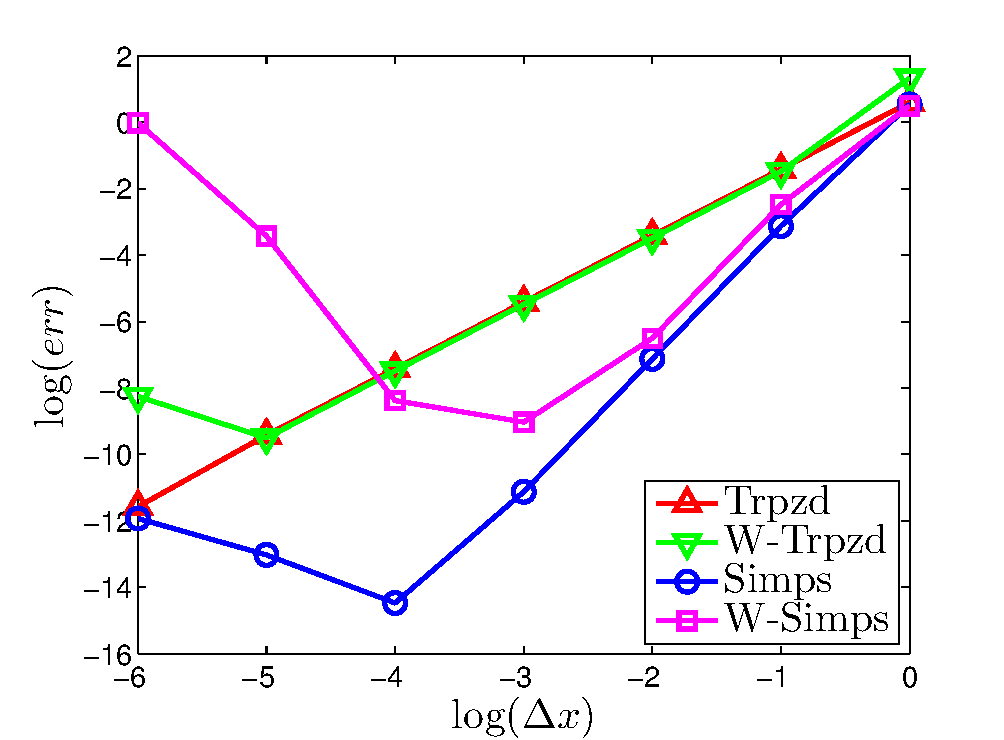
\includegraphics[width=0.5\textwidth]{wtws}
  \caption{Numerical integrations of Slater-Condon parameters with $k=6$ for hydrogen wave
  function ``$4f$'' using trapezoidal, weighted-trapezoidal, Simpson and weighted Simpson's rules.
  This figure plots the relative error against the grid size $\Delta x$ on a log-log scale.}
  \label{fig:wtws}
\end{figure}

However, the weighted integration methods do not give a better accuracy. On the contrary,
the accuracy is worse than a traditional numerical integration scheme. The problem was caused
by the ``division by a very small number'' numerical error. In the coefficients $\alpha$, $\beta$
and $\gamma$, we had some terms like $1/(k^3\Delta x^2)$. If $\Delta x$ goes very small, say,
$10^{-6}$, a large numerical error could be introduced due to machine accuracy.
Although we have spent so much effort deriving the weighted integration method, we would still
stick with the traditional Simpson's rule as our integration method. On the other hand, this
is also a ``good news'' as the Simpson's rule is much easier to implement.

If we are only interested in the electron interactions in the same shell,
i.e.\ $n_1l_1=n_2l_2=n_3l_3=n_4l_4=nl$, Eqn.~(\ref{eq:RkSplit}) simplifies to
\begin{equation} \label{eq:Fk}
F^{(k)}(nl) =
\int_0^\infty dr_1 |u_{nl}(r_1)|^2
\left[ \frac{1}{r_1^{k+1}} \int_0^{r_1} dr_2\, r_2^k |u_{nl}(r_2)|^2
+ r_1^k \int_{r_1}^\infty dr_2\, \frac{1}{r_2^{k+1}} |u_{nl}(r_2)|^2 \right]
\end{equation}
%
To verify the accuracy of Simpson's integration on the Slater-Condon parameters,
we take the first few hydrogen wave functions as inputs, which are known exactly.
We compute the on-shell interaction parameters according to Eqn.~(\ref{eq:Fk}).
We used a grid $\{r_\text{min}=0.0001;r_\text{max}=150.0;\Delta x=0.002;\}$.\footnote{We
used a grid wider than (\ref{eq:grid}) to be able to represent hydrogen wave functions
with large principle quantum numbers, which spread out to the further region from the nucleus.}
The results are listed in Table~\ref{table:slater}. Notice that exact wave functions
are used as input. In practical calculations, when a numerical wave function is provided,
the results will be subject to the accuracy of the given numerical wave function.

\begin{table}[h!]
\caption{Numerical (Simpson's rule) and exact Slater-Condon parameters
for the first few exact hydrogen wave functions. Energies are given in units of
Hartree (a.u.).}
\label{table:slater}
\begin{center}
\begin{tabular}{ c | c | c | c | c | c }
  \hline
 Orbital &$k$ & Numerical  &  Exact     & Abs Error  & Rel Error \\ \hline \hline
 $1s$    &  0 &  0.625000  &  $5/8\phantom{00}$           &  $2.7842\times10^{-12}$  &  $4.4547\times10^{-12}$ \\ \hline
 $2s$    &  0 &  0.150391  &  $77/512\phantom{0}$         &  $2.1716\times10^{-13}$  &  $1.4440\times10^{-12}$ \\ \hline
 $2p$    &  0 &  0.181641  &  $93/512\phantom{0}$         &  $7.8798\times10^{-14}$  &  $4.3381\times10^{-13}$ \\ 
         &  2 &  0.087891  &  $45/512\phantom{0}$         &  $3.0531\times10^{-14}$  &  $3.4738\times10^{-13}$ \\ \hline
 $3s$    &  0 &  0.066406  &  $17/256\phantom{0}$         &  $1.4978\times10^{-13}$  &  $2.2556\times10^{-12}$ \\ \hline
 $3p$    &  0 &  0.071868  &  $1987/27648\phantom{0}$     &  $1.1495\times10^{-13}$  &  $1.5995\times10^{-12}$ \\ 
         &  2 &  0.035988  &  $995/27648$                 &  $3.9472\times10^{-13}$  &  $1.0968\times10^{-11}$ \\ \hline
 $3d$    &  0 &  0.086046  &  $793/9216\phantom{0}$       &  $6.3449\times10^{-14}$  &  $7.3739\times10^{-13}$ \\ 
         &  2 &  0.045421  &  $2093/46080\phantom{0}$     &  $1.1700\times10^{-13}$  &  $2.5760\times10^{-12}$ \\ 
         &  4 &  0.029622  &  $91/3072$                   &  $6.3165\times10^{-13}$  &  $2.1323\times10^{-11}$ \\ \hline
 $4s$    &  0 &  0.037271  &  $19541/524288\phantom{0}$   &  $1.4345\times10^{-13}$  &  $3.8489\times10^{-12}$ \\ \hline
 $4p$    &  0 &  0.038935  &  $20413/524288\phantom{0}$   &  $1.2726\times10^{-13}$  &  $3.2685\times10^{-12}$ \\ 
         &  2 &  0.019922  &  $10445/524288\phantom{0}$   &  $5.2667\times10^{-13}$  &  $2.6436\times10^{-11}$ \\ \hline
 $4d$    &  0 &  0.042673  &  $22373/524288\phantom{0}$   &  $9.9913\times10^{-14}$  &  $2.3414\times10^{-12}$ \\ 
         &  2 &  0.021573  &  $56553/2621440$             &  $3.8654\times10^{-13}$  &  $1.7917\times10^{-11}$ \\ 
         &  4 &  0.014780  &  $7749/524288$               &  $2.2203\times10^{-13}$  &  $1.5022\times10^{-11}$ \\ \hline
 $4f$    &  0 &  0.050226  &  $26333/524288\phantom{0}$   &  $5.4602\times10^{-14}$  &  $1.0871\times10^{-12}$ \\ 
         &  2 &  0.028140  &  $103275/3670016\phantom{0}$ &  $1.4186\times10^{-13}$  &  $5.0413\times10^{-12}$ \\ 
         &  4 &  0.018802  &  $69003/3670016$             &  $2.9456\times10^{-13}$  &  $1.5667\times10^{-11}$ \\ 
         &  6 &  0.013910  &  $7293/524288$               &  $1.6736\times10^{-12}$  &  $1.2031\times10^{-10}$ \\
  \hline
\end{tabular}
\end{center}
\end{table}

\section{Gaunt coefficients}
Our next task is to solve the angular part:
\begin{align} \label{eq:Ak}
A^{(k)}(l_1m_1,l_2m_2,l_3m_3,l_4m_4) = \sum_{\mu=-k}^k
& \int_0^{2\pi}d\phi_1 \int_0^{\pi}d\theta_1\,\sin{\theta_1}\,
  \conj{Y_{l_1m_1}}(\theta_1,\phi_1) \conj{Y_{k\mu}}(\theta_1,\phi_1) Y_{l_4m_4}(\theta_1,\phi_1) \nonumber \\
& \int_0^{2\pi}d\phi_2 \int_0^{\pi}d\theta_2\,\sin{\theta_2}\,
  \conj{Y_{l_2m_2}}(\theta_2,\phi_2) Y_{k\mu}(\theta_2,\phi_2) Y_{l_3m_3}(\theta_2,\phi_2)
\end{align}
%
Our life simplifies in Bra-Ket notation:
\begin{equation} \label{eq:AkBK}
A^{(k)}(l_1m_1,l_2m_2,l_3m_3,l_4m_4) = \sum_{\mu=-k}^k \Bra{l_1m_1} \conj{k\mu} \Ket{l_4m_4} \Bra{l_2m_2} k\mu \Ket{l_3m_3}
\end{equation}
%
We can get rid of the complex conjugate in the middle by using an important relation
of spherical harmonics:\footnote{You see, we put a comma to
separate indices when there is an ambiguity. While $k\mu$ appears as two indices,
the notation $k{-\mu}$ looks like ``$k$ minus $\mu$''. For the later case, we prefer $k,-\mu$
to make it clear.}
\begin{equation} \label{eq:YY}
\conj{Y_{k\mu}}(\theta,\phi) = (-1)^{\mu} Y_{k,-\mu}(\theta,\phi)
\end{equation}
%
Now Eqn.~(\ref{eq:AkBK}) becomes,
\begin{equation} \label{eq:AkBKm}
A^{(k)}(l_1m_1,l_2m_2,l_3m_3,l_4m_4) = \sum_{\mu=-k}^k (-1)^{\mu} \Bra{l_1m_1} k,-\mu \Ket{l_4m_4} \Bra{l_2m_2} k\mu \Ket{l_3m_3}
\end{equation}
%
A term like $\Bra{l_1m_1} k\mu \Ket{l_2m_2}$ is called a Gaunt coefficient.
It is purely integrals of three spherical harmonics. An important property of
this integral is that the integration vanishes under certain combinations of
indices. Non-trivial Gaunt coefficients must satisfy the sum rules:
\begin{equation} \label{eq:muRule}
\mu = m_1 - m_2
\end{equation}
\begin{equation} \label{eq:kRule}
|l_1-l_2| \le k \le l_1+l_2 \quad \text{and} \quad l_1+l_2+k \text{ is even}
\end{equation}
%
While the relation in Eqn.~(\ref{eq:kRule}) is difficult to derive,
it is rather straightforward to show the sum rule in Eqn.~(\ref{eq:muRule}).
One can express the spherical harmonics in terms of the associated Legendre
polynomials,\footnote{The associated Legendre polynomials are defined as
$P_l^m(x) = (-1)^m (1-x^2)^{m/2} \frac{d^m}{dx^m}(P_l(x))$.}
\begin{equation} \label{eq:spha}
Y_{lm}(\theta,\phi) = \sqrt{\frac{2l+1}{4\pi}\frac{(l-m)!}{(l+m)!}} e^{im\phi} P_l^m(\cos{\theta})
\end{equation}
Therefore, a Gaunt coefficient reads,
\begin{align} \label{eq:muRuleShow}
\Bra{l_1m_1} k\mu \Ket{l_2m_2} =
{} & \sqrt{\frac{(2l_1+1)(2k+1)(2l_2+1)}{(4\pi)^3}
\frac{(l_1-m_1)!(k-\mu)!(l_2-m_2)!}{(l_1+m_1)!(k+\mu)!(l_2+m_2)!}} \nonumber \\
& \int_0^{2\pi}d\phi\, e^{i\phi(-m_1+\mu+m_2)}
\int_0^{\pi}d\theta\,\sin{\theta}\,
P_{l_1}^{m_1}(\cos{\theta}) P_k^\mu(\cos{\theta}) P_{l_2}^{m_2}(\cos{\theta})
\end{align}
It can be seen that if $-m_1+\mu+m_2 \ne 0$, the $\phi$ integral from 0 to
$2\pi$ over a complex exponential function gives 0. Hence we had Eqn.~(\ref{eq:muRule}).
It is also important to notice that the Gaunt coefficients are real numbers.
Now we use a notation for Gaunt coefficients
\begin{equation} \label{eq:gnt}
g_{m_1m_2}^{(k)} = \Bra{l_1m_1} k\mu \Ket{l_2m_2}
\end{equation}
We dropped indices $l_1$ and $l_2$ in the notation $g_{m_1m_2}^{(k)}$
because they are usually predefined.
We also dropped the index $\mu$ since it is determined by $m_1$ and $m_2$
automatically. Because of this uniqueness of $\mu$, only one term
survives in the summations in Eqn.~(\ref{eq:AkBKm}).
\begin{equation} \label{eq:AkBKone}
\boxed{A^{(k)}(l_1m_1,l_2m_2,l_3m_3,l_4m_4) = (-1)^{\mu} g_{m_1m_4}^{(k)} g_{m_2m_3}^{(k)}}
\end{equation}
%
It is now a matter of evaluating the Gaunt coefficients. The integration of
three spherical harmonics can be obtained from a recursion relation.
\begin{equation} \label{eq:GauntRec}
\Bra{l_1m_1} k\mu \Ket{l_2m_2} = a \Bra{l_1+1,m_1} k-1,\mu \Ket{l_2m_2}
+ b \Bra{l_1-1,m_1} k-1,\mu \Ket{l_2m_2}
+ c \Bra{l_1m_1} k-2,\mu \Ket{l_2m_2}
\end{equation}
where,
\begin{align}
a & = \sqrt{\frac{(2k+1)(2k-1)(l_1+m_1+1)(l_1-m_1+1)}{(k+\mu)(k-\mu)(2l_1+3)(2l_1+1)}} \label{eq:afact} \\
b & = \sqrt{\frac{(2k+1)(2k-1)(l_1+m_1)(l_1-m_1)}{(k+\mu)(k-\mu)(2l_1+1)(2l_1-1)}} \label{eq:bfact} \\
c & = -\sqrt{\frac{(2k+1)(k+\mu-1)(k-\mu-1)}{(k+\mu)(k-\mu)(2k-3)}} \label{eq:cfact}
\end{align}
with base case,
\begin{equation} \label{eq:GauntBase}
\Bra{l_1m_1} 00 \Ket{l_2m_2} = \frac{1}{\sqrt{4\pi}} \delta_{l_1l_2} \delta_{m_1m_2}
\end{equation}

\paragraph{Derivation:}
Warning: A bit long.

Given the relation between $Y_{lm}$ and $P_l^m$
and the recursion relation of the associated Legendre polynomials,
\begin{equation} \label{eq:PtoY}
Y_{lm} = \sqrt{\frac{2l+1}{4\pi}\frac{(l-m)!}{(l+m)!}} e^{im\phi} P_l^m
\end{equation}
\begin{equation} \label{eq:Prec}
(l-m+1)P_{l+1}^m = (2l+1)xP_l^m - (l+m)P_{l-1}^m
\end{equation}
We get,
\begin{equation} \label{eq:Yrec}
(l-m+1)\sqrt{\frac{(2l+1)(l+m+1)}{(2l+3)(l-m+1)}} Y_{l+1,m} = (2l+1)xY_{lm} - (l+m)\sqrt{\frac{(2l+1)(l-m)}{(2l-1)(l+m)}} Y_{l-1,m}
\end{equation}
Now, substitutions,\footnote{Notice that the following
notations are equivalent: $\Bra{Y_{l_1m_1}}Y_{k\mu}\Ket{Y_{l_2m_2}} = \Bra{l_1m_1}k\mu\Ket{l_2m_2}$.
Here we prefer the former one, since a term like ``$xY_{lm}$'' is less confusing than
``$xlm$''}
\begin{align}
& \Bra{Y_{l_1m_1}} \boxed{Y_{k\mu}} \Ket{Y_{l_2m_2}} \nonumber \\
= {} & \Bra{Y_{l_1m_1}} \frac{1}{k-\mu}\sqrt{\frac{(2k+1)(k-\mu)}{(2k-1)(k+\mu)}}
\left[ (2k-1)xY_{k-1,\mu} - (k+\mu-1)\sqrt{\frac{(2k-1)(k-\mu-1)}{(2k-3)(k+\mu-1)}}Y_{k-2,\mu} \right]
\Ket{Y_{l_2m_2}} \nonumber \\
= {} & \sqrt{\frac{(2k+1)(2k-1)}{(k+\mu)(k-\mu)}}
\boxed{\Bra{xY_{l_1m_1}}} Y_{k-1,\mu} \Ket{Y_{l_2m_2}}
-\sqrt{\frac{(2k+1)(k+\mu-1)(k-\mu-1)}{(k+\mu)(k-\mu)(2k-3)}}
\Bra{Y_{l_1m_1}} Y_{k-2,\mu} \Ket{Y_{l_2m_2}} \nonumber \\
= {} & \sqrt{\frac{(2k+1)(2k-1)}{(k+\mu)(k-\mu)}} \left[
\frac{l_1-m_1+1}{2l_1+1}\sqrt{\frac{(2l_1+1)(l_1+m_1+1)}{(2l_1+3)(l_1-m_1+1)}}
\Bra{Y_{l_1+1,m_1}} Y_{k-1,\mu} \Ket{Y_{l_2m_2}} \right. \nonumber \\
& \left. + \frac{l_1+m_1}{2l_1+1}\sqrt{\frac{(2l_1+1)(l_1-m_1)}{(2l_1-1)(l_1+m_1)}}
\Bra{Y_{l_1-1,m_1}} Y_{k-1,\mu} \Ket{Y_{l_2m_2}} \right] \nonumber \\
& -\sqrt{\frac{(2k+1)(k+\mu-1)(k-\mu-1)}{(k+\mu)(k-\mu)(2k-3)}}
\Bra{Y_{l_1m_1}} Y_{k-2,\mu} \Ket{Y_{l_2m_2}} \nonumber \\
= {} & \sqrt{\frac{(2k+1)(2k-1)(l_1+m_1+1)(l_1-m_1+1)}{(k+\mu)(k-\mu)(2l_1+3)(2l_1+1)}}
\Bra{Y_{l_1+1,m_1}} Y_{k-1,\mu} \Ket{Y_{l_2m_2}} \nonumber \\
& + \sqrt{\frac{(2k+1)(2k-1)(l_1+m_1)(l_1-m_1)}{(k+\mu)(k-\mu)(2l_1+1)(2l_1-1)}}
\Bra{Y_{l_1-1,m_1}} Y_{k-1,\mu} \Ket{Y_{l_2m_2}} \nonumber \\
& -\sqrt{\frac{(2k+1)(k+\mu-1)(k-\mu-1)}{(k+\mu)(k-\mu)(2k-3)}}
\Bra{Y_{l_1m_1}} Y_{k-2,\mu} \Ket{Y_{l_2m_2}} \qquad \text{Q.E.D.}
\end{align}

To get a flavor of how this recursion works, we consider an element
\begin{equation*}
\Bra{1,-1} 2,0 \Ket{1,-1}
\end{equation*}
Apply Eqn.~(\ref{eq:GauntRec}), we find
\begin{align}
& \Bra{1,-1} 2,0 \Ket{1,-1} \nonumber \\
= & {} \frac{\sqrt{3}}{2} \Bra{2,-1} 1,0 \Ket{1,-1}
+ 0 \underbrace{\Bra{0,-1}}_{\text{undefined}} 1,0 \Ket{1,-1}
- \frac{\sqrt{5}}{2} \underbrace{\Bra{1,-1} 0,0 \Ket{1,-1}}_{1/\sqrt{4\pi}} \nonumber \\
= & {} \frac{\sqrt{3}}{2} \left(
\sqrt{\frac{24}{35}}\underbrace{\Bra{3,-1} 0,0 \Ket{1,-1}}_{0}
+ \sqrt{\frac{3}{5}}\underbrace{\Bra{1,-1} 0,0 \Ket{1,-1}}_{1/\sqrt{4\pi}}
+ 0\Bra{2,-1} \underbrace{-1,0}_{\text{undefined}} \Ket{1,-1} \right) - \frac{\sqrt{5}}{2\sqrt{4\pi}} \nonumber \\
= & {} -\frac{1}{\sqrt{20\pi}}
\end{align}
Yeah, we found it!

Recursion (\ref{eq:GauntRec}) is universal for all Gaunt coefficients. So one
would expect that we could implement a recursive function
\texttt{Gaunt(l1, l2, k, m1, m2)}
and apply to every Gaunt to obtain their values. That would be too good
to be true. Unfortunately, our recursive function can only be used
for the diagonal elements (strictly speaking, for $m_1=m_2$).
Now consider,
\begin{equation*}
\Bra{1,-1} 2,-2 \Ket{1,1}
\end{equation*}
Apply Eqn.~(\ref{eq:GauntRec}),
\begin{align}
& \Bra{1,-1} 2,-2 \Ket{1,1} \nonumber \\
= & {} \sqrt{\frac{30}{0}} \Bra{2,-1} \underbrace{1,-2}_{\text{undefined}} \Ket{1,1}
+ \sqrt{\frac{0}{0}} \underbrace{\Bra{0,-1} 1,-2}_{\text{undefined}} \Ket{1,1}
- \sqrt{\frac{-15}{0}} \Bra{1,-1} \underbrace{0,-2}_{\text{undefined}} \Ket{1,1} \nonumber \\
= & {} \text{NaN}
\end{align}
Not-a-Number.

This doesn't mean that $\Bra{1,-1} 2,-2 \Ket{1,1}$ is equal to
infinity or zero or what. A ratio $0/0$ can give us anything, but the information
is destroyed. We cannot extract this value from recursion (\ref{eq:GauntRec}).
This ``division by zeros'' problem is caused by a non-zero $\mu$, namely, $m_1 \ne m_2$.
The term $(k+\mu)(k-\mu)$ in the denominator becomes zero if $|\mu|=k$.
To get the off-diagonal elements, we have to ask help from the ladder operators
$L_+$ and $L_-$. Recall,
\begin{equation} \label{eq:ladder}
L_\pm \Ket{lm} = \alpha_{lm}^\pm \Ket{l,m\pm1}
\end{equation}
where,
\begin{align}
\alpha_{lm}^+ & = \sqrt{(l+m+1)(l-m)} \label{eq:ldalphaUp} \\
\alpha_{lm}^- & = \sqrt{(l+m)(l-m+1)} \label{eq:ldalphaDn}
\end{align}
%
Now consider two nonzero elements
\begin{equation*}
\Big( \Bra{l_1m_1} L_+ \Big) k,\mu-1 \Ket{l_2m_2}
\quad \text{and} \quad
\Big( \Bra{l_1m_1} L_- \Big) k,\mu+1 \Ket{l_2m_2}
\end{equation*}
%
\begin{equation} \label{eq:ladderUp}
\begin{cases}
\Big( \Bra{l_1m_1} L_+ \Big) k,\mu-1 \Ket{l_2m_2} = \alpha_{l_1m_1}^- \Bra{l_1,m_1-1} k,\mu-1 \Ket{l_2m_2} \\
\Bra{l_1m_1} \Big( L_+\, k,\mu-1 \Ket{l_2m_2} \Big) = \alpha_{k,\mu-1}^+ \Bra{l_1m_1} k\mu \Ket{l_2m_2} + \alpha_{l_2m_2}^+ \Bra{l_1m_1} k,\mu-1 \Ket{l_2,m_2+1}
\end{cases}
\end{equation}
\begin{equation} \label{eq:ladderDn}
\begin{cases}
\Big( \Bra{l_1m_1} L_- \Big) k,\mu+1 \Ket{l_2m_2} = \alpha_{l_1m_1}^+ \Bra{l_1,m_1+1} k,\mu+1 \Ket{l_2m_2} \\
\Bra{l_1m_1} \Big( L_-\, k,\mu+1 \Ket{l_2m_2} \Big) = \alpha_{k,\mu+1}^- \Bra{l_1m_1} k\mu \Ket{l_2m_2} + \alpha_{l_2m_2}^- \Bra{l_1m_1} k,\mu+1 \Ket{l_2,m_2-1}
\end{cases}
\end{equation}
%
From Eqn.~(\ref{eq:ladderUp}), we get the relation
\begin{equation} \label{eq:ldUp}
\alpha_{l_1m_1}^- \Bra{l_1,m_1-1} k,\mu-1 \Ket{l_2m_2} =
\alpha_{k,\mu-1}^+ \Bra{l_1m_1} k\mu \Ket{l_2m_2} + \alpha_{l_2m_2}^+ \Bra{l_1m_1} k,\mu-1 \Ket{l_2,m_2+1}
\end{equation}
which binds three Gaunt coefficients as
\begin{equation*}
\begin{bmatrix}
\cdots & \cdots & \cdots & \cdots \\
\cdots & \boxed{g_{m_1-1,m_2}} & g_{m_1-1,m_2+1} & \cdots \\
\cdots & \boxed{g_{m_1,\phantom{-1}m_2}} & \boxed{g_{m_1,\phantom{-1}m_2+1}} & \cdots \\
\cdots & \cdots & \cdots & \cdots
\end{bmatrix}
\end{equation*}
%
From Eqn.~(\ref{eq:ladderDn}), we get the relation
\begin{equation} \label{eq:ldDn}
\alpha_{l_1m_1}^+ \Bra{l_1,m_1+1} k,\mu+1 \Ket{l_2m_2} =
\alpha_{k,\mu+1}^- \Bra{l_1m_1} k\mu \Ket{l_2m_2} + \alpha_{l_2m_2}^- \Bra{l_1m_1} k,\mu+1 \Ket{l_2,m_2-1}
\end{equation}
which binds three Gaunt coefficients as
\begin{equation*}
\begin{bmatrix}
\cdots & \cdots & \cdots & \cdots \\
\cdots & \boxed{g_{m_1,\phantom{+1}m_2-1}} & \boxed{g_{m_1,\phantom{+1}m_2}} & \cdots \\
\cdots & g_{m_1+1,m_2-1} & \boxed{g_{m_1+1,m_2}} & \cdots \\
\cdots & \cdots & \cdots & \cdots
\end{bmatrix}
\end{equation*}
%
As an illustration, we consider the Gaunt coefficient matrix for $l_1=1$ and
$l_2=2$. This matrix has the following rectangular shape:
\begin{equation*}
\begin{blockarray}{cccccc}
  & -2 & -1 & \ 0 & \ 1 & \ 2 \\
\begin{block}{c[ccccc]}
 -1 & \ \phantom{0,} & \ \phantom{0,} & \ \phantom{0,} & \ \phantom{0,} & \ \phantom{0,} \\
\phantom{-}0 &  &  &  &  &  \\
\phantom{-}1 &  &  &  &  &  \\
\end{block}
\end{blockarray}
\end{equation*}
where the $m_1$ index traverses vertically (row number) and the $m_2$ index
traverses horizontally (column number). A simple strategy for calculating the matrix
elements is shown in the diagram below
\begin{equation*}
\begin{blockarray}{cccccc}
  & -2 & -1 & \ 0 & \ 1 & \ 2 \\
\begin{block}{c[ccccc]}
 -1 & \leftarrow & \otimes & \rightarrow & \rightarrow & \rightarrow \\
\phantom{-}0 & \leftarrow & \leftarrow & \otimes & \rightarrow & \rightarrow \\
\phantom{-}1 & \leftarrow & \leftarrow & \leftarrow & \otimes & \rightarrow \\
\end{block}
\end{blockarray}
\end{equation*}
The elements ``$\otimes$'' are the diagonal elements with $m_1=m_2$,
which can be calculated directly from the recursion relation. The arrows
indicate the direction of applying the ladder operator relations.
Notice that any element outside the matrix is zero, because
the coefficients $\alpha_{lm}^\pm$ in (\ref{eq:ldalphaUp})
and (\ref{eq:ldalphaDn}) vanish for $m=l$ and $-l$, respectively.
A detailed pictorial illustration is shown below: (play it as an animation, once an elements is
calculated, we stamp an $\otimes$)
\begin{equation*}
\begin{blockarray}{ccccc}
  \boxed{0} &  &  &  &  \\
\begin{block}{[ccccc]}
  \boxed{?} & \boxed{\otimes} &  &  &  \\
   &  & \otimes &  &  \\
 \phantom{\boxed{\otimes}} & \phantom{\otimes} & \phantom{\otimes} & \otimes & \phantom{\otimes} \\
\end{block}
\end{blockarray}
\begin{blockarray}{ccccc}
   & \boxed{0} &  &  &  \\
\begin{block}{[ccccc]}
  \otimes & \boxed{\otimes} & \boxed{?} &  &  \\
   &  & \otimes &  &  \\
 \phantom{\otimes} & \phantom{\otimes} & \phantom{\boxed{\otimes}} & \otimes & \phantom{\otimes} \\
\end{block}
\end{blockarray}
\begin{blockarray}{ccccc}
   &  & \boxed{0} &  &  \\
\begin{block}{[ccccc]}
  \otimes & \otimes & \boxed{\otimes} & \boxed{?} &  \\
   &  & \otimes &  &  \\
 \phantom{\otimes} & \phantom{\otimes} & \phantom{\boxed{\otimes}} & \otimes & \phantom{\otimes} \\
\end{block}
\end{blockarray}
\begin{blockarray}{ccccc}
   &  &  & \boxed{0}  &  \\
\begin{block}{[ccccc]}
  \otimes & \otimes & \otimes & \boxed{\otimes} & \boxed{?}  \\
  \phantom{\otimes} & \phantom{\otimes} & \otimes & \phantom{\boxed{\otimes}} & \phantom{\otimes} \\
   &  &  & \otimes &  \\
\end{block}
\end{blockarray}
\end{equation*}
\begin{equation*}
\begin{blockarray}{ccccc}
\begin{block}{[ccccc]}
 \otimes & \boxed{\otimes} & \otimes & \otimes & \otimes \\
  & \boxed{?} & \boxed{\otimes} &  &  \\
  &  &  & \otimes &  \\
\end{block}
\end{blockarray}
\begin{blockarray}{ccccc}
\begin{block}{[ccccc]}
 \boxed{\otimes} & \otimes & \otimes & \otimes & \otimes \\
 \boxed{?} & \boxed{\otimes} & \otimes &  &  \\
  &  &  & \otimes &  \\
\end{block}
\end{blockarray}
\begin{blockarray}{ccccc}
\begin{block}{[ccccc]}
  \otimes & \otimes & \boxed{\otimes} & \otimes & \otimes \\
  \otimes & \otimes & \boxed{\otimes} & \boxed{?} &  \\
   &  &   & \otimes &  \\
\end{block}
\end{blockarray}
\begin{blockarray}{ccccc}
\begin{block}{[ccccc]}
  \otimes & \otimes & \otimes & \boxed{\otimes} & \otimes \\
  \otimes & \otimes & \otimes & \boxed{\otimes} & \boxed{?} \\
   &  &  & \otimes &  \\
\end{block}
\end{blockarray}
\end{equation*}
\begin{equation*}
\begin{blockarray}{ccccc}
\begin{block}{[ccccc]}
  \otimes & \otimes & \otimes & \otimes & \otimes \\
  \otimes & \otimes & \boxed{\otimes} & \otimes & \otimes \\
  &  & \boxed{?} & \boxed{\otimes} &  \\
\end{block}
\end{blockarray}
\begin{blockarray}{ccccc}
\begin{block}{[ccccc]}
  \otimes & \otimes & \otimes & \otimes & \otimes \\
  \otimes & \boxed{\otimes} & \otimes & \otimes & \otimes \\
  & \boxed{?} & \boxed{\otimes} & \otimes &  \\
\end{block}
\end{blockarray}
\begin{blockarray}{ccccc}
\begin{block}{[ccccc]}
  \otimes & \otimes & \otimes & \otimes & \otimes \\
  \boxed{\otimes} & \otimes & \otimes & \otimes & \otimes \\
  \boxed{?} & \boxed{\otimes} & \otimes & \otimes &  \\
\end{block}
\end{blockarray}
\begin{blockarray}{ccccc}
\begin{block}{[ccccc]}
  \otimes & \otimes & \otimes & \otimes & \otimes \\
  \otimes & \otimes & \otimes & \boxed{\otimes} & \otimes \\
  \otimes & \otimes & \otimes & \boxed{\otimes} & \boxed{?} \\
\end{block}
\end{blockarray}
\end{equation*}
Complete! The speed of the algorithm can be doubled
if we consider the symmetry of the matrix. (remember that Gaunt coefficients
are real)
\begin{align} \label{eq:GauntSymm}
\Bra{l_1m_1}k\mu\Ket{l_2m_2}
& = (-1)^{m_1+m_2+\mu} \Bra{\conj{l_1,-m_1}}\conj{k,-\mu}\Ket{\conj{l_2,-m_2}} \nonumber \\
& = (-1)^{2m_1} \conj{\Bra{\conj{l_1,-m_1}}\conj{k,-\mu}\Ket{\conj{l_2,-m_2}}} \nonumber \\
& = \Bra{l_1,-m_1}k,-\mu\Ket{l_2,-m_2}
\end{align}
%
Eqn.~(\ref{eq:GauntSymm}) says, the Gaunt matrix has the following symmetry: (inverse symmetry)
\begin{equation*}
\begin{blockarray}{cccccc}
  & -2 & -1 & \ 0\ & \ 1\ & \ 2\ \\
\begin{block}{c[ccccc]}
 -1 & \ominus & \times & \heartsuit & + & \diamondsuit \\
\phantom{-}0 & \div & \triangle & \odot & \triangle & \div \\
\phantom{-}1 & \diamondsuit & + & \heartsuit & \times & \ominus \\
\end{block}
\end{blockarray}
\end{equation*}
%
Hence, our algorithm simplifies to:
\begin{equation*}
\begin{blockarray}{ccccc}
   & \boxed{0} &  &  &  \\
\begin{block}{[ccccc]}
   & \boxed{\otimes} & \boxed{?} &  &  \\
   &  & \otimes &  &  \\
 \phantom{\otimes} & \phantom{\otimes} & ? & \otimes & \phantom{\otimes} \\
\end{block}
\end{blockarray}
\begin{blockarray}{ccccc}
   &  & \boxed{0} &  &  \\
\begin{block}{[ccccc]}
   & \otimes & \boxed{\otimes} & \boxed{?} &  \\
   &  & \otimes &  &  \\
 \phantom{\otimes} & ? & \otimes & \otimes & \phantom{\otimes} \\
\end{block}
\end{blockarray}
\begin{blockarray}{ccccc}
   &  &  & \boxed{0}  &  \\
\begin{block}{[ccccc]}
   & \otimes & \otimes & \boxed{\otimes} & \boxed{?}  \\
   &  & \otimes &  &  \\
  ? & \otimes & \otimes & \otimes & \phantom{\otimes} \\
\end{block}
\end{blockarray}
\end{equation*}
\begin{equation*}
\begin{blockarray}{ccccc}
\begin{block}{[ccccc]}
   & \otimes & \boxed{\otimes} & \otimes & \otimes \\
   & ? & \boxed{\otimes} & \boxed{?} &  \\
  \otimes & \otimes & \otimes & \otimes & \phantom{\otimes} \\
\end{block}
\end{blockarray}
\begin{blockarray}{ccccc}
\begin{block}{[ccccc]}
   & \otimes & \otimes & \boxed{\otimes} & \otimes \\
  ? & \otimes & \otimes & \boxed{\otimes} & \boxed{?} \\
  \otimes & \otimes & \otimes & \otimes & \phantom{\otimes} \\
\end{block}
\end{blockarray}
\begin{blockarray}{ccccc}
\begin{block}{[ccccc]}
  ? & \otimes & \otimes & \otimes & \otimes \\
  \otimes & \otimes & \otimes & \boxed{\otimes} & \otimes \\
  \otimes & \otimes & \otimes & \boxed{\otimes} & \boxed{?} \\
\end{block}
\end{blockarray}
\end{equation*}
Done! Symmetry in Eqn.~(\ref{eq:GauntSymm}) allows us to compute just half of the
elements thus obtaining a speed up. Yet, there is another symmetry property
of Gaunt coefficients which relates two adjoint matrices. (Gaunt coefficients
are real)
\begin{align} \label{eq:GauntAdjt}
\Bra{l_1m_1}k\mu\Ket{l_2m_2}
& = \conj{\Bra{l_1m_1}k\mu\Ket{l_2m_2}} \nonumber \\
& = \Bra{l_2m_2}\conj{k\mu}\Ket{l_1m_1} \nonumber \\
& = (-1)^\mu\Bra{l_2m_2}k,-\mu\Ket{l_1m_1}
\end{align}
%
Eqn.~(\ref{eq:GauntAdjt}) says,
\begin{equation*}
\begin{bmatrix}
  \otimes & \otimes & \otimes & \boxed{\otimes} & \otimes \\
  \otimes & \otimes & \otimes & \otimes & \otimes \\
  \otimes & \otimes & \otimes & \otimes & \otimes
\end{bmatrix}
\longleftrightarrow
\begin{bmatrix}
  \oplus & \oplus & \oplus \\
  \oplus & \oplus & \oplus \\
  \oplus & \oplus & \oplus \\
  \boxed{\oplus} & \oplus & \oplus \\
  \oplus & \oplus & \oplus
\end{bmatrix}
\quad
\text{where, }
\boxed{\oplus} = (-1)^\mu\boxed{\otimes}
\end{equation*}
%
Once the Gaunt matrix with $l_1=1$ and $l_2=2$ is determined, the Gaunt
matrix with $l_1=2$ and $l_2=1$ can be read off directly without doing another calculation.

Previously, we calculated all diagonal elements from the recursion relation.
That was absolutely valid, but recursive calls may cost considerable
computational time especially when the matrix gets huge.
In fact, we need to calculate only one diagonal element from the
recursion relation. The others can be obtained from ladder operators.
For example (a 5-by-7 matrix):
\begin{equation*}
\begin{bmatrix}
  & \otimes &  &  &  &  & \\
  &  &  &  &  &  & \\
  &  &  &  &  &  & \\
  &  &  &  &  &  & \\
  \phantom{\otimes} & \phantom{\otimes} & \phantom{\otimes} & \phantom{\otimes} & \phantom{\otimes} & \otimes & \phantom{\otimes}
\end{bmatrix}
\begin{bmatrix}
   & \otimes & \otimes & \otimes & \otimes & \otimes & \otimes \\
   &  &  &  &  &  & \\
   &  &  &  &  &  & \\
   &  &  &  &  &  & \\
  \otimes & \otimes & \otimes & \otimes & \otimes & \otimes & 
\end{bmatrix}
\begin{bmatrix}
   & \boxed{\otimes} & \boxed{\otimes} & \otimes & \otimes & \otimes & \otimes \\
   &  & \boxed{?} &  &  &  & \\
   &  &  &  &  &  & \\
   &  &  &  & ? &  & \\
  \otimes & \otimes & \otimes & \otimes & \otimes & \otimes & 
\end{bmatrix}
\end{equation*}
\begin{equation*}
\begin{bmatrix}
   & \otimes & \otimes & \otimes & \otimes & \otimes & \otimes \\
   &  & \otimes &  &  &  & \\
   &  &  &  &  &  & \\
   &  &  &  & \otimes &  & \\
  \otimes & \otimes & \otimes & \otimes & \otimes & \otimes & 
\end{bmatrix}
\begin{bmatrix}
   & \otimes & \otimes & \otimes & \otimes & \otimes & \otimes \\
   &  & \otimes & \otimes & \otimes & \otimes & \otimes \\
   &  &  &  &  &  & \\
  \otimes & \otimes & \otimes & \otimes & \otimes &  & \\
  \otimes & \otimes & \otimes & \otimes & \otimes & \otimes & 
\end{bmatrix}
\begin{bmatrix}
   & \otimes & \otimes & \otimes & \otimes & \otimes & \otimes \\
   &  & \boxed{\otimes} & \boxed{\otimes} & \otimes & \otimes & \otimes \\
   &  &  & \boxed{?} &  &  & \\
  \otimes & \otimes & \otimes & \otimes & \otimes &  & \\
  \otimes & \otimes & \otimes & \otimes & \otimes & \otimes & 
\end{bmatrix}
\end{equation*}
\begin{equation*}
\begin{bmatrix}
   & \otimes & \otimes & \otimes & \otimes & \otimes & \otimes \\
   &  & \otimes & \otimes & \otimes & \otimes & \otimes \\
   &  &  & \otimes &  &  & \\
  \otimes & \otimes & \otimes & \otimes & \otimes &  & \\
  \otimes & \otimes & \otimes & \otimes & \otimes & \otimes & 
\end{bmatrix}
\begin{bmatrix}
   & \otimes & \otimes & \otimes & \otimes & \otimes & \otimes \\
   &  & \otimes & \otimes & \otimes & \otimes & \otimes \\
  \otimes & \otimes & \otimes & \otimes & \otimes & \otimes & \otimes \\
  \otimes & \otimes & \otimes & \otimes & \otimes &  & \\
  \otimes & \otimes & \otimes & \otimes & \otimes & \otimes & 
\end{bmatrix}
\begin{bmatrix}
  \otimes & \,\otimes & \,\otimes & \,\,\otimes & \,\otimes & \,\otimes & \,\otimes \\
  \otimes & \,\otimes & \,\otimes & \,\,\otimes & \,\otimes & \,\otimes & \,\otimes \\
  \otimes & \,\otimes & \,\otimes & \,\,\otimes & \,\otimes & \,\otimes & \,\otimes \\
  \otimes & \,\otimes & \,\otimes & \,\,\otimes & \,\otimes & \,\otimes & \,\otimes \\
  \otimes & \,\otimes & \,\otimes & \,\,\otimes & \,\otimes & \,\otimes & \,\otimes
\end{bmatrix}
\end{equation*}

This is how we implement our program to evaluate the Gaunt coefficients.
It might be useful if we summarize a few Gaunt matrices with $l_1=l_2$ for $s$,
$p$, $d$ and $f$ shells (the on-shell interactions). The results are listed in the
next pages.

\newpage
$s$ shell ($l_1=l_2=0$):

$k=0$
\begin{equation} \label{eq:Gstart}
\frac{1}{\sqrt{4\pi}}
\begin{bmatrix*}[r]
1
\end{bmatrix*}
\end{equation}

$p$ shell ($l_1=l_2=1$):

$k=0$
\begin{equation}
\phantom{\frac{1}{\sqrt{5}}} \frac{1}{\sqrt{4\pi}}
\begin{bmatrix*}[r]
\phantom{000}1 & \,\phantom{000}0 & \,\phantom{000}0 \\
0 & 1 & 0 \\
0 & 0 & 1
\end{bmatrix*}
\end{equation}

$k=2$
\begin{equation}
\frac{1}{\sqrt{4\pi}} \frac{1}{\sqrt{5}}
\begin{bmatrix*}[r]
-1 & \phantom{-}\sqrt{3} & -\sqrt{6} \\
-\sqrt{3} & 2 & -\sqrt{3} \\
-\sqrt{6} & \sqrt{3} & -1
\end{bmatrix*}
\end{equation}

$d$ shell ($l_1=l_2=2$):

$k=0$
\begin{equation}
\phantom{\frac{1}{7}} \frac{1}{\sqrt{4\pi}}
\begin{bmatrix*}[r]
\phantom{0000}1 & \,\phantom{0000}0 & \,\phantom{0000}0 & \,\phantom{0000}0 & \,\phantom{0000}0 \\
0 & 1 & 0 & 0 & 0 \\
0 & 0 & 1 & 0 & 0 \\
0 & 0 & 0 & 1 & 0 \\
0 & 0 & 0 & 0 & 1
\end{bmatrix*}
\end{equation}

$k=2$
\begin{equation}
\frac{1}{\sqrt{4\pi}} \frac{1}{7}
\begin{bmatrix*}[r]
-\sqrt{20} & \sqrt{30} & -\sqrt{20} & 0 & 0 \\ 
-\sqrt{30} & \sqrt{5} & \sqrt{5} & -\sqrt{30} & 0 \\ 
-\sqrt{20} & -\sqrt{5} & \sqrt{20} & -\sqrt{5} & -\sqrt{20} \\ 
0 & -\sqrt{30} & \sqrt{5} & \sqrt{5} & -\sqrt{30} \\ 
0 & 0 & -\sqrt{20} & \sqrt{30} & -\sqrt{20}
\end{bmatrix*}
\end{equation}

$k=4$
\begin{equation}
\frac{1}{\sqrt{4\pi}} \frac{1}{7}
\begin{bmatrix*}[r]
1 & -\sqrt{5} & \sqrt{15} & -\sqrt{35} & \phantom{-}\sqrt{70} \\ 
\sqrt{5} & -4 & \sqrt{30} & -\sqrt{40} & \sqrt{35} \\ 
\sqrt{15} & -\sqrt{30} & 6 & -\sqrt{30} & \sqrt{15} \\ 
\sqrt{35} & -\sqrt{40} & \sqrt{30} & -4 & \sqrt{5} \\ 
\phantom{-}\sqrt{70} & -\sqrt{35} & \phantom{-}\sqrt{15} & -\sqrt{5} & 1
\end{bmatrix*}
\end{equation}

\newpage
$f$ shell ($l_1=l_2=3$):

$k=0$
\begin{equation}
\phantom{\frac{5}{33\sqrt{13}}} \frac{1}{\sqrt{4\pi}}
\begin{bmatrix*}[r]
\phantom{-\sqrt{00}}1 & 0 & 0 & 0 & 0 & 0 & 0 \\
0 & \phantom{-\sqrt{00}}1 & 0 & 0 & 0 & 0 & 0 \\
0 & 0 & \phantom{-\sqrt{00}}1 & 0 & 0 & 0 & 0 \\
0 & 0 & 0 & \phantom{-\sqrt{00}}1 & 0 & 0 & 0 \\
0 & 0 & 0 & 0 & \phantom{-\sqrt{00}}1 & 0 & 0 \\
0 & 0 & 0 & 0 & 0 & \phantom{-\sqrt{00}}1 & 0 \\
0 & 0 & 0 & 0 & 0 & 0 & \phantom{-\sqrt{00}}1
\end{bmatrix*}
\end{equation}

$k=2$
\begin{equation}
\phantom{00} \frac{1}{\sqrt{4\pi}} \frac{1}{3\sqrt{5}}
\begin{bmatrix*}[r]
-5 & 5 & -\sqrt{10} & 0 & 0 & 0 & 0 \\ 
-5 & 0 & \sqrt{15} & \phantom{0}{-\sqrt{20}} & 0 & 0 & 0 \\ 
\phantom{0}{-\sqrt{10}} & \phantom{0}{-\sqrt{15}} & 3 & \sqrt{2} & \phantom{0}{-\sqrt{24}} & 0 & 0 \\ 
0 & -\sqrt{20} & -\sqrt{2} & 4 & -\sqrt{2} & \phantom{0}{-\sqrt{20}} & 0 \\ 
0 & 0 & \phantom{0}{-\sqrt{24}} & \sqrt{2} & 3 & -\sqrt{15} & \phantom{0}{-\sqrt{10}} \\ 
0 & 0 & 0 & -\sqrt{20} & \sqrt{15} & 0 & -5 \\ 
0 & 0 & 0 & 0 & -\sqrt{10} & 5 & -5
\end{bmatrix*}
\end{equation}

$k=4$
\begin{equation}
\phantom{000,} \frac{1}{\sqrt{4\pi}} \frac{1}{11}
\begin{bmatrix*}[r]
3 & -\sqrt{30} & \sqrt{54} & -\sqrt{63} & \sqrt{42} & 0 & 0 \\ 
\sqrt{30} & -7 & \sqrt{32} & -\sqrt{3} & -\sqrt{14} & \sqrt{70} & 0 \\ 
\phantom{-0}\sqrt{54} & \phantom{0}{-\sqrt{32}} & 1 & \phantom{-0}\sqrt{15} & \phantom{0}{-\sqrt{40}} & \phantom{-0}\sqrt{14} & \phantom{-0}\sqrt{42} \\ 
\sqrt{63} & -\sqrt{3} & \phantom{0}{-\sqrt{15}} & 6 & -\sqrt{15} & -\sqrt{3} & \sqrt{63} \\ 
\sqrt{42} & \sqrt{14} & -\sqrt{40} & \sqrt{15} & 1 & -\sqrt{32} & \sqrt{54} \\ 
0 & \sqrt{70} & -\sqrt{14} & -\sqrt{3} & \sqrt{32} & -7 & \sqrt{30} \\ 
0 & 0 & \sqrt{42} & -\sqrt{63} & \sqrt{54} & -\sqrt{30} & 3
\end{bmatrix*}
\end{equation}

$k=6$
\begin{equation} \label{eq:Gend}
\frac{1}{\sqrt{4\pi}} \frac{5}{33\sqrt{13}}
\begin{bmatrix*}[r]
-1 & \sqrt{7} & -\sqrt{28} & \sqrt{84} & -\sqrt{210} & \sqrt{462} & -\sqrt{924} \\
-\sqrt{7} & 6 & -\sqrt{105} & \sqrt{224} & -\sqrt{378} & \sqrt{504} & -\sqrt{462} \\
-\sqrt{28} & \phantom{-}\sqrt{105} & -15 & \phantom{-}\sqrt{350} & -\sqrt{420} & \phantom{-}\sqrt{378} & -\sqrt{210} \\
-\sqrt{84} & \sqrt{224} & -\sqrt{350} & 20 & -\sqrt{350} & \sqrt{224} & -\sqrt{84} \\
-\sqrt{210} & \sqrt{378} & -\sqrt{420} & \sqrt{350} & -15 & \sqrt{105} & -\sqrt{28} \\
-\sqrt{462} & \sqrt{504} & -\sqrt{378} & \sqrt{224} & -\sqrt{105} & 6 & -\sqrt{7} \\
-\sqrt{924} & \sqrt{462} & -\sqrt{210} & \sqrt{84} & -\sqrt{28} & \sqrt{7} & -1
\end{bmatrix*}
\end{equation}
